% Options for packages loaded elsewhere
\PassOptionsToPackage{unicode}{hyperref}
\PassOptionsToPackage{hyphens}{url}
%
\documentclass[
  ignorenonframetext,
]{beamer}
\usepackage{pgfpages}
\setbeamertemplate{caption}[numbered]
\setbeamertemplate{caption label separator}{: }
\setbeamercolor{caption name}{fg=normal text.fg}
\beamertemplatenavigationsymbolsempty
% Prevent slide breaks in the middle of a paragraph
\widowpenalties 1 10000
\raggedbottom
\setbeamertemplate{part page}{
  \centering
  \begin{beamercolorbox}[sep=16pt,center]{part title}
    \usebeamerfont{part title}\insertpart\par
  \end{beamercolorbox}
}
\setbeamertemplate{section page}{
  \centering
  \begin{beamercolorbox}[sep=12pt,center]{part title}
    \usebeamerfont{section title}\insertsection\par
  \end{beamercolorbox}
}
\setbeamertemplate{subsection page}{
  \centering
  \begin{beamercolorbox}[sep=8pt,center]{part title}
    \usebeamerfont{subsection title}\insertsubsection\par
  \end{beamercolorbox}
}
\AtBeginPart{
  \frame{\partpage}
}
\AtBeginSection{
  \ifbibliography
  \else
    \frame{\sectionpage}
  \fi
}
\AtBeginSubsection{
  \frame{\subsectionpage}
}
\usepackage{amsmath,amssymb}
\usepackage{iftex}
\ifPDFTeX
  \usepackage[T1]{fontenc}
  \usepackage[utf8]{inputenc}
  \usepackage{textcomp} % provide euro and other symbols
\else % if luatex or xetex
  \usepackage{unicode-math} % this also loads fontspec
  \defaultfontfeatures{Scale=MatchLowercase}
  \defaultfontfeatures[\rmfamily]{Ligatures=TeX,Scale=1}
\fi
\usepackage{lmodern}
\usetheme[]{AnnArbor}
\usecolortheme{dolphin}
\usefonttheme{structurebold}
\ifPDFTeX\else
  % xetex/luatex font selection
\fi
% Use upquote if available, for straight quotes in verbatim environments
\IfFileExists{upquote.sty}{\usepackage{upquote}}{}
\IfFileExists{microtype.sty}{% use microtype if available
  \usepackage[]{microtype}
  \UseMicrotypeSet[protrusion]{basicmath} % disable protrusion for tt fonts
}{}
\makeatletter
\@ifundefined{KOMAClassName}{% if non-KOMA class
  \IfFileExists{parskip.sty}{%
    \usepackage{parskip}
  }{% else
    \setlength{\parindent}{0pt}
    \setlength{\parskip}{6pt plus 2pt minus 1pt}}
}{% if KOMA class
  \KOMAoptions{parskip=half}}
\makeatother
\usepackage{xcolor}
\newif\ifbibliography
\usepackage{graphicx}
\makeatletter
\def\maxwidth{\ifdim\Gin@nat@width>\linewidth\linewidth\else\Gin@nat@width\fi}
\def\maxheight{\ifdim\Gin@nat@height>\textheight\textheight\else\Gin@nat@height\fi}
\makeatother
% Scale images if necessary, so that they will not overflow the page
% margins by default, and it is still possible to overwrite the defaults
% using explicit options in \includegraphics[width, height, ...]{}
\setkeys{Gin}{width=\maxwidth,height=\maxheight,keepaspectratio}
% Set default figure placement to htbp
\makeatletter
\def\fps@figure{htbp}
\makeatother
\setlength{\emergencystretch}{3em} % prevent overfull lines
\providecommand{\tightlist}{%
  \setlength{\itemsep}{0pt}\setlength{\parskip}{0pt}}
\setcounter{secnumdepth}{-\maxdimen} % remove section numbering

\usepackage{amsmath}
\usepackage{nomencl}
\makenomenclature 


%\usepackage{booktabs}
%\usepackage{longtable}
%\usepackage{morefloats}
%\extrafloats{100}
%\date{August 25, 2021}
%\renewcommand{\today}{September 5, 2021}

% Set the copyright footer
%\lfoot{\copyright 2021 P.J. Palmer  P.M. Leonard}

% Some figure placement options.
%\usepackage[figuresonly,nomarkers,fighead, figlist]{endfloat}
%\usepackage[figuresonly,nomarkers,nolists]{endfloat}
% Put multiple figures per page
%\renewcommand{\efloatseparator}{\mbox{}}

\usepackage{caption}
\captionsetup[figure]{labelformat=empty}
\ifLuaTeX
  \usepackage{selnolig}  % disable illegal ligatures
\fi
\IfFileExists{bookmark.sty}{\usepackage{bookmark}}{\usepackage{hyperref}}
\IfFileExists{xurl.sty}{\usepackage{xurl}}{} % add URL line breaks if available
\urlstyle{same}
\hypersetup{
  pdftitle={Identifying Those Tricky Little Micro-moths},
  pdfauthor={Paul J. Palmer},
  hidelinks,
  pdfcreator={LaTeX via pandoc}}

\title{Identifying Those Tricky Little Micro-moths}
\author{Paul J. Palmer}
\date{}

\begin{document}
\frame{\titlepage}

\begin{frame}{What Is A Micro-moth?}
\protect\hypertarget{what-is-a-micro-moth}{}
\begin{itemize}
\tightlist
\item
  This is a tricky question to answer as there no taxonomic difference,
  as in butterflies and moths. Even that is a bit blurred.
\item
  So far as I can tell, the larger moths are those that were described
  in South vols 1 and 2, and the rest are the micro-moths.
\item
  In the olden days when we used a light trap there we so many large
  moths that we were never tempted by the micro's that were trampled by
  the Noctua pronuba (Large Yellow Underwing) which came in their
  hundreds.
\item
  Micro's were collected by rearing out series collected off food plants
  and mines.
\item
  The first (and current) editions of ``The Field Guide To The Smaller
  Lepidoptera'' contains no illustrations of adult moths at all.
\end{itemize}
\end{frame}

\begin{frame}{Wot! No Illustrations?}
\protect\hypertarget{wot-no-illustrations}{}
Don't worry, I will use them later in this presentation.

\begin{itemize}
\tightlist
\item
  Without illustrations the emphasis for identification rested on
  descriptions of the larval behaviour and food plants plus the overall
  appearance of the adult being consistent with the overall family and
  genus of the specimen.
\item
  Just to emphasise, you had to be really proficient with your plant
  identification too.
\item
  My old copy of Clapham, Tutin, and Warburgh ``The Excursion Flora Of
  The British Isle'' was also without images.
\item
  To those of you only used to modern illustrated field guides this must
  sound very strange, but the point I make is that a good identification
  is based on a collection of evidence which is used to eliminate all
  but one possibility.
\end{itemize}
\end{frame}

\begin{frame}{First Steps}
\protect\hypertarget{first-steps}{}
\begin{columns}[T]
\begin{column}{0.5\textwidth}
\begin{itemize}
\tightlist
\item
  Light traps catch fewer moths these days, so the micro-moths are more
  obvious.
\item
  The publication of the excellent illustrated `Field Guide to the
  Micro-Moths of Great Britain and Ireland' has helped popularise this
  group further.
\item
  BUT, the temptation for beginners is to `pattern match' from a field
  guide.
\item
  The availability of `Apps' reinforces this approach.
\end{itemize}
\end{column}

\begin{column}{0.5\textwidth}
\begin{figure}
\centering
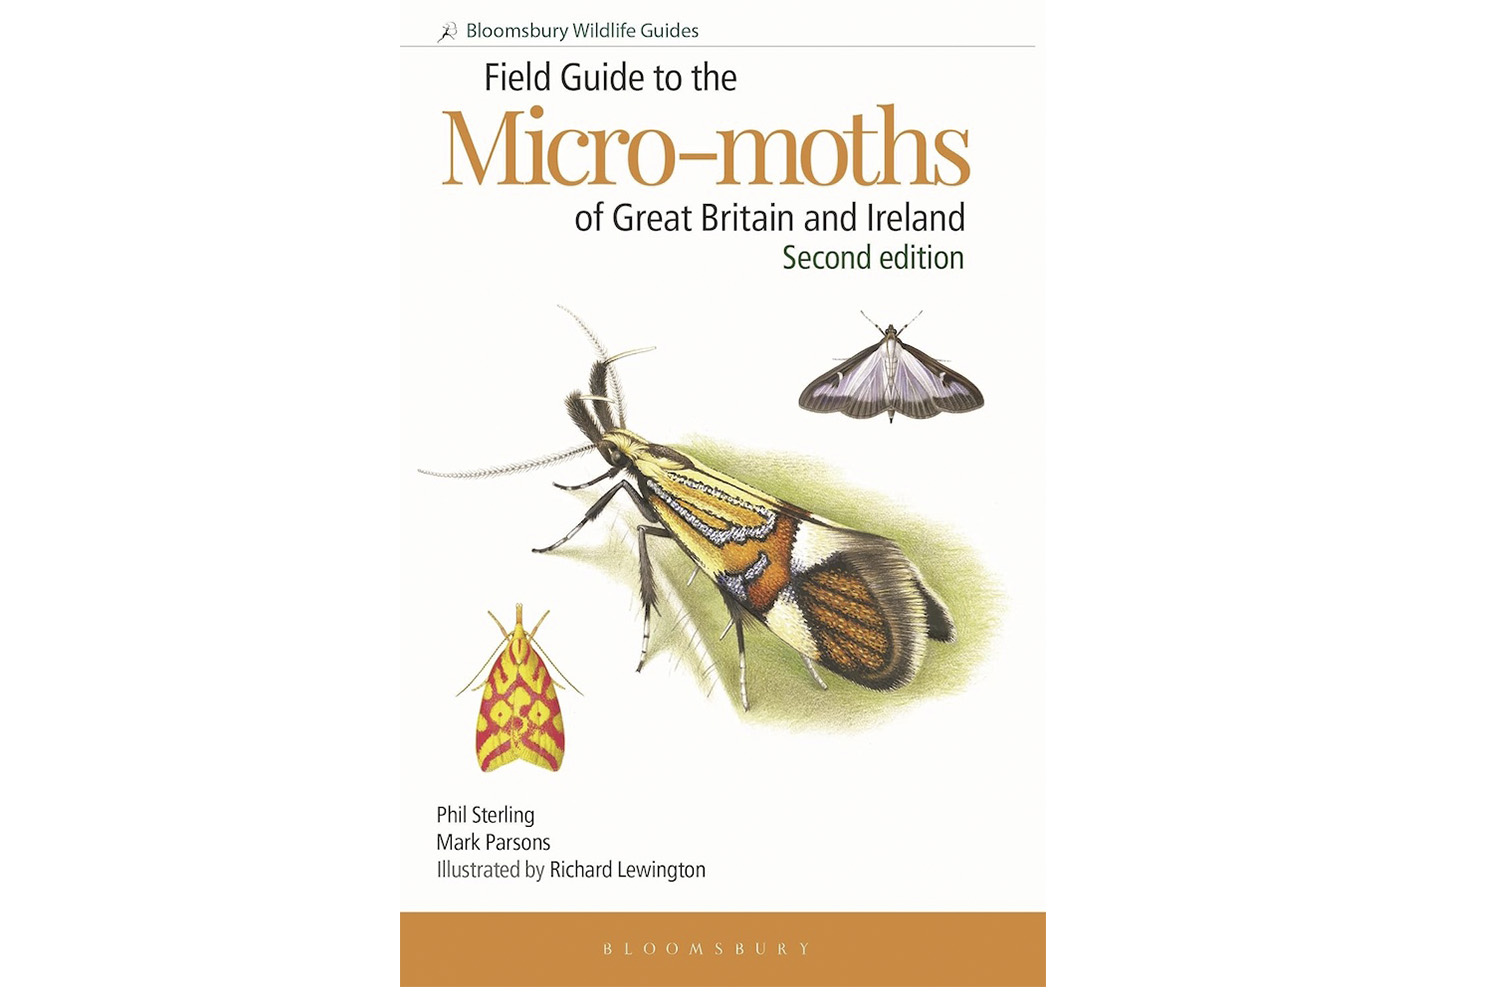
\includegraphics{./images/micro-field-guide.jpg}
\caption{Field Guide to the Micro Moths}
\end{figure}
\end{column}
\end{columns}
\end{frame}

\begin{frame}{Identification Is A Process}
\protect\hypertarget{identification-is-a-process}{}
\begin{columns}[T]
\begin{column}{0.5\textwidth}
\begin{itemize}
\tightlist
\item
  Examine your specimen closely.
\item
  Treat ID as process and start by writing down everything that you know
  and can see.
\item
  Use these notes to try and work out the Family.
\item
  There is a good visual key to families in `Field Guide to the
  Micro-Moths of Great Britain and Ireland'.
\item
  Lepidoptera keys to species level are few and far between.
\end{itemize}
\end{column}

\begin{column}{0.5\textwidth}
\begin{figure}
\centering
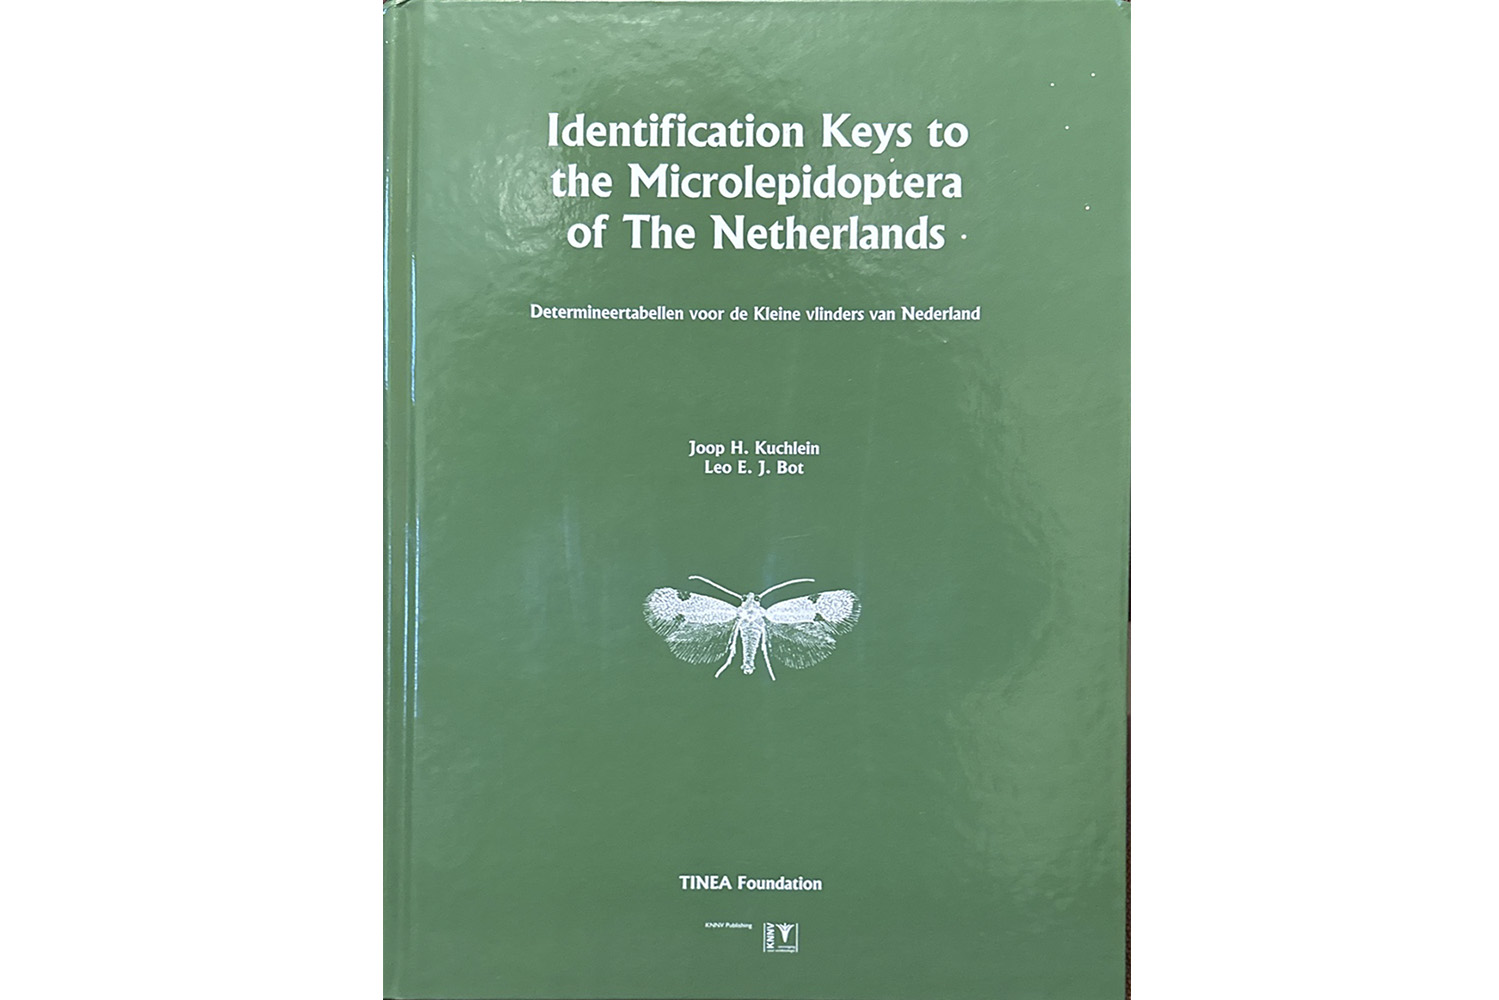
\includegraphics{./images/micro-lep-key.jpg}
\caption{A key to the Micro Moths}
\end{figure}
\end{column}
\end{columns}
\end{frame}

\begin{frame}{A Tricky Moth For ID}
\protect\hypertarget{a-tricky-moth-for-id}{}
\begin{columns}[T]
\begin{column}{0.5\textwidth}
\begin{itemize}
\tightlist
\item
  Making a list of candidate species is a tedious and time-consuming
  process.
\item
  You should now have a list that includes: size, locality and type of
  habitat; date; and other obvious features.
\item
  A photograph is also helpful - look at the posture and position of the
  antennae.
\end{itemize}
\end{column}

\begin{column}{0.5\textwidth}
\begin{figure}
\centering
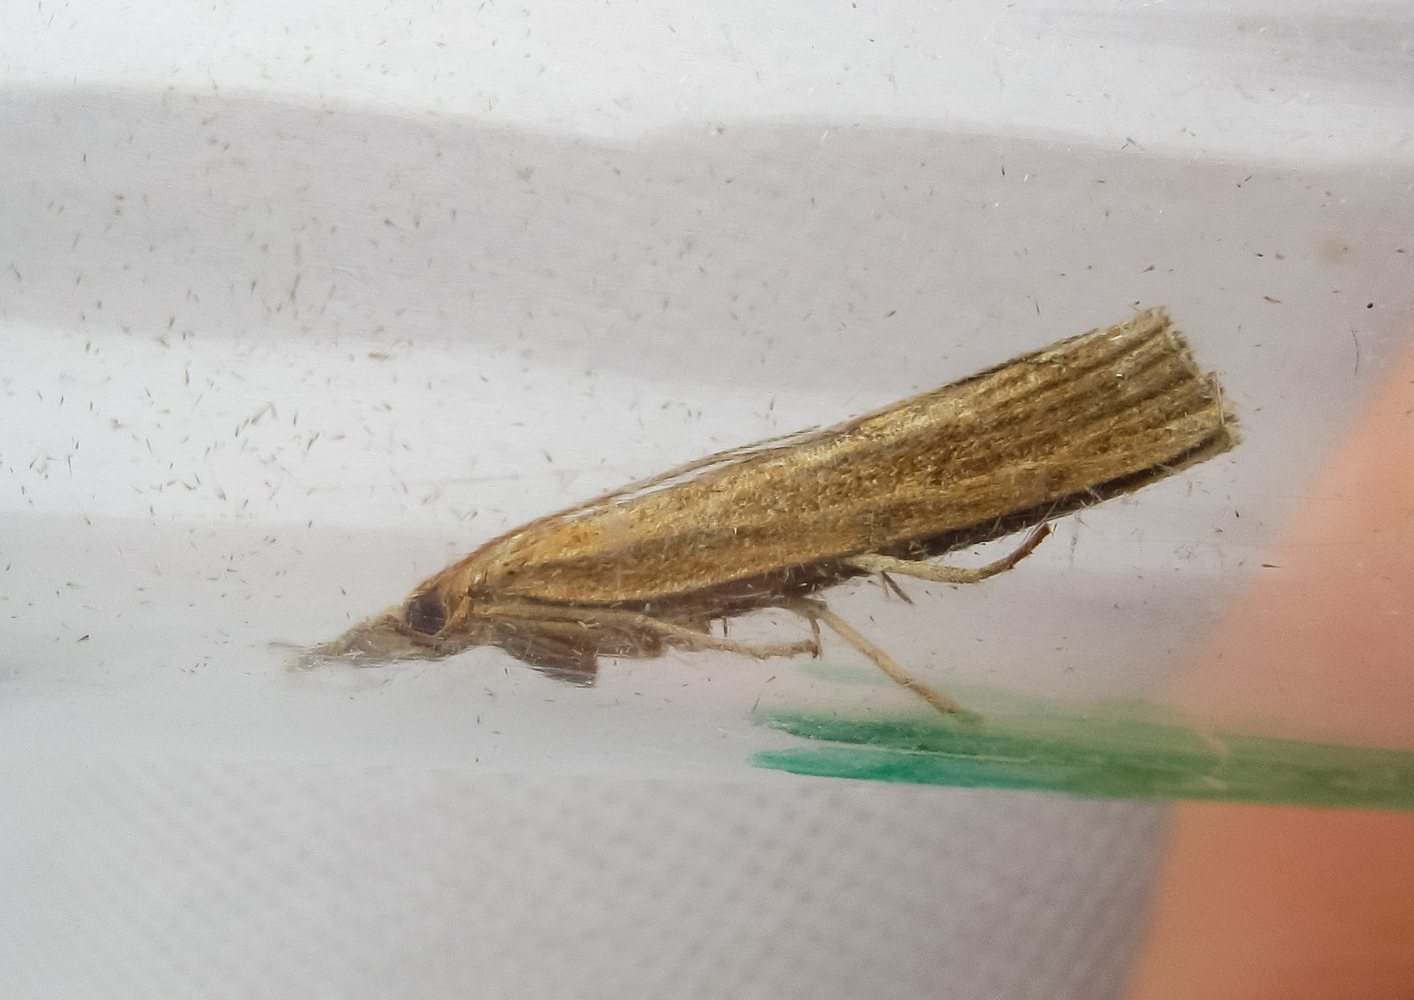
\includegraphics{./images/Pcontaminella-PML-2021.jpg}
\caption{What can we see here?}
\end{figure}
\end{column}
\end{columns}

We will illustrate the ID process by following one moth tricky moth
through its journey.
\end{frame}

\begin{frame}{Checking The Basics}
\protect\hypertarget{checking-the-basics}{}
\begin{columns}[T]
\begin{column}{0.5\textwidth}
\begin{itemize}
\tightlist
\item
  First check that our specimen is a moth.
\item
  This is not as daft as it sounds as it is not unheard of for a Caddis
  (Order: Trichoptera) to be queried as a moth.
\item
  In this case the overall appearance is definitely Lepidoptera.
\end{itemize}
\end{column}

\begin{column}{0.5\textwidth}
\begin{figure}
\centering
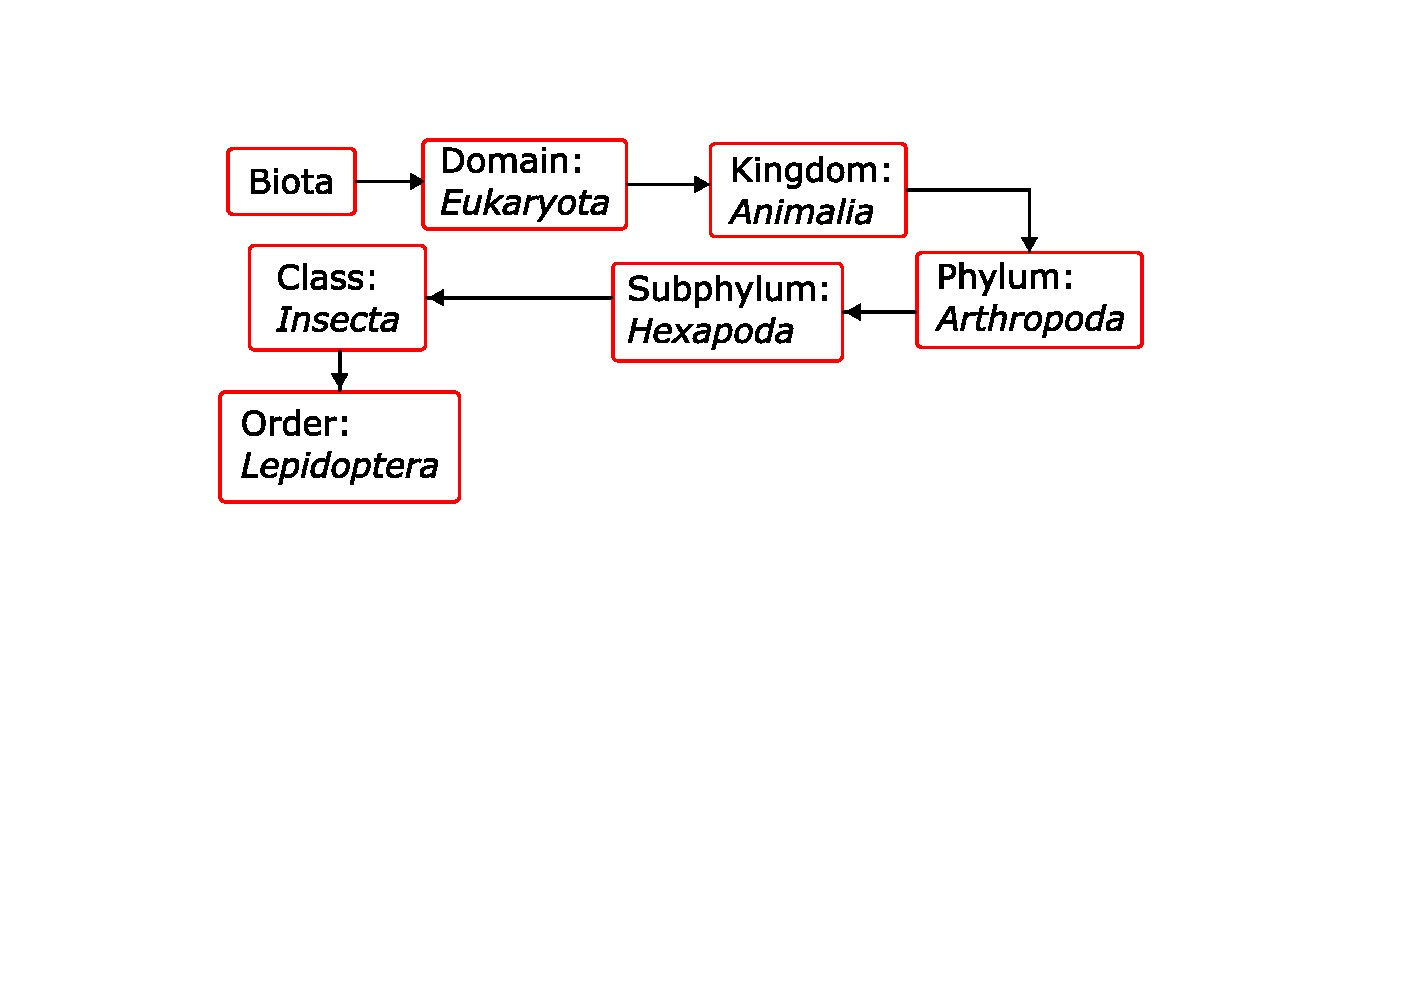
\includegraphics{./images/order.jpg}
\caption{Tree of life (biology)}
\end{figure}
\end{column}
\end{columns}
\end{frame}

\begin{frame}{Checking External Features}
\protect\hypertarget{checking-external-features}{}
\begin{columns}[T]
\begin{column}{0.5\textwidth}
\begin{itemize}
\tightlist
\item
  All the short jawed Lepidoptera are micro moths, so it is quite likely
  that you will come across them, especially those that might be tricky
  to ID.
\item
  This specimen has a long coiled tongue, rather than short jaws, as
  have the majority of the Lepidoptera.
\item
  The long long coiled tongue means that this moth is a member of the
  \textbf{Glossata}.
\end{itemize}
\end{column}

\begin{column}{0.5\textwidth}
\begin{figure}
\centering
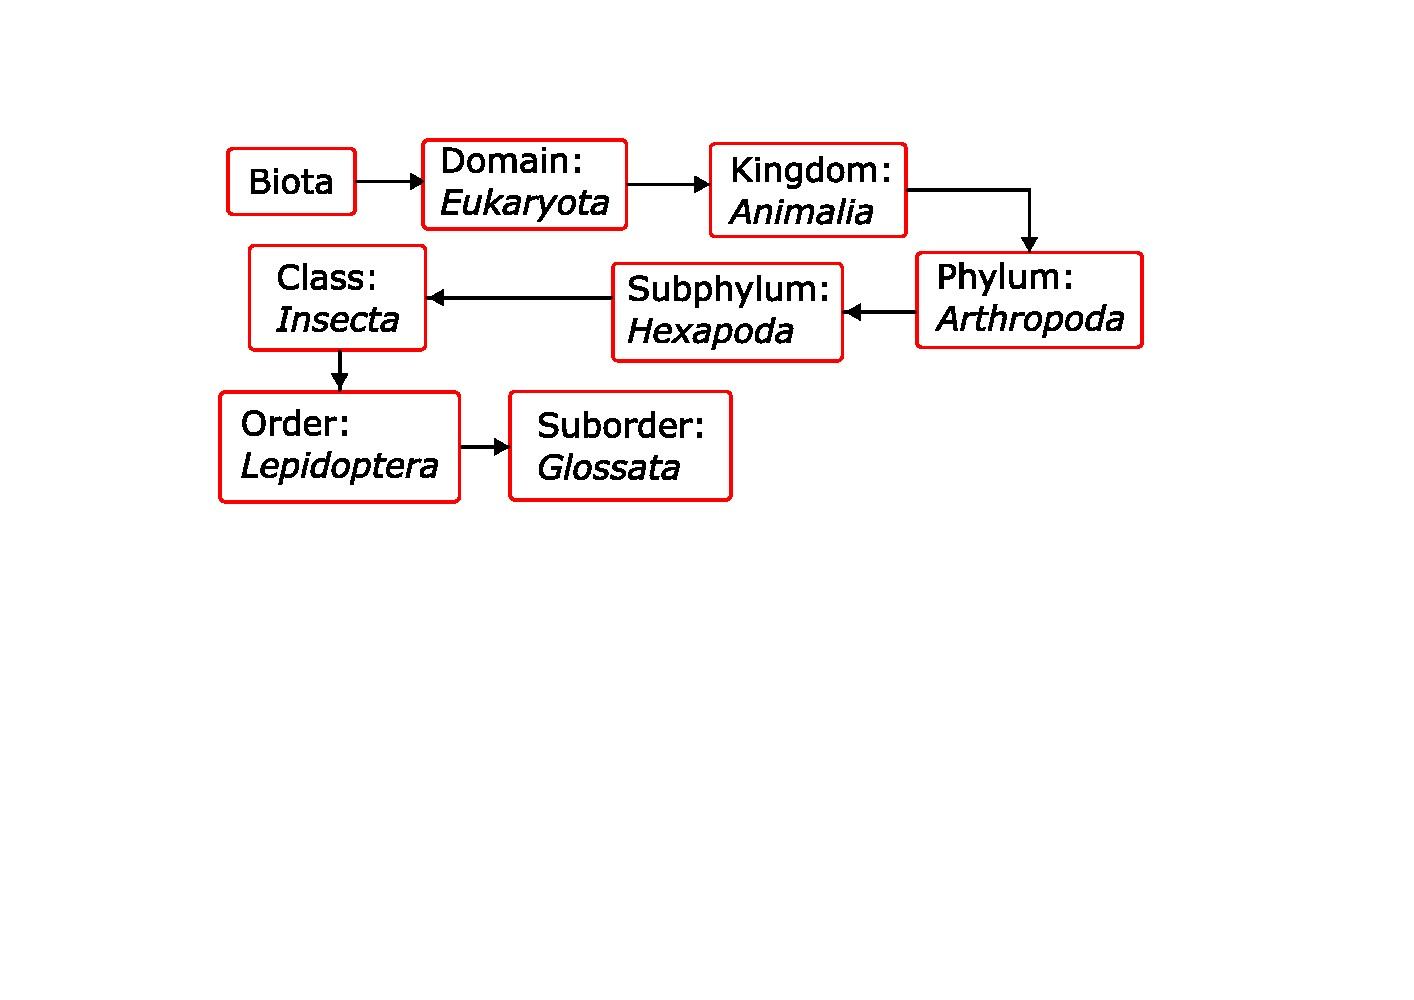
\includegraphics{./images/suborder.jpg}
\caption{Tree of life (biology)}
\end{figure}
\end{column}
\end{columns}
\end{frame}

\begin{frame}{Getting To The Family}
\protect\hypertarget{getting-to-the-family}{}
\begin{columns}[T]
\begin{column}{0.5\textwidth}
\begin{itemize}
\tightlist
\item
  The face has a distinctive `nose' and face. Also the antennae are
  laying flush along the body:
\item
  This is a member of the \textbf{Pyraloidea} super-family.
\end{itemize}
\end{column}

\begin{column}{0.5\textwidth}
\begin{figure}
\centering
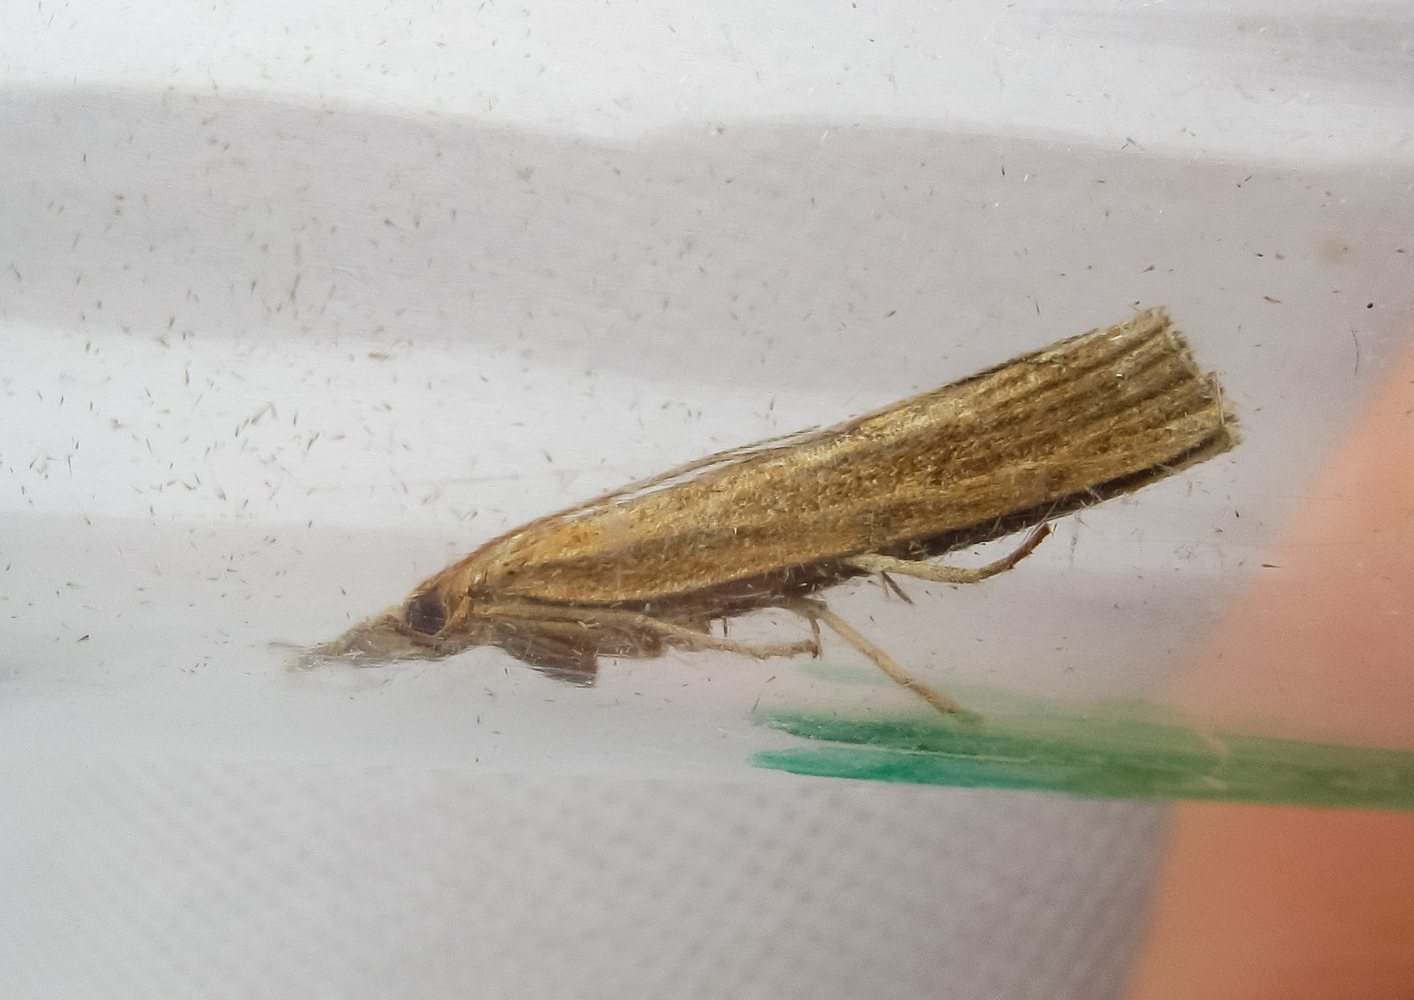
\includegraphics{./images/Pcontaminella-PML-2021.jpg}
\caption{Note the posture.}
\end{figure}
\end{column}
\end{columns}
\end{frame}

\begin{frame}{Following Branches Of The Tree}
\protect\hypertarget{following-branches-of-the-tree}{}
\begin{columns}[T]
\begin{column}{0.5\textwidth}
\begin{itemize}
\tightlist
\item
  Now, the \textbf{Crambidae} family are very variable, but this moth is
  a member of the subfamily \textbf{Crambinae}, as the long wings can
  wrap tightly around the body. Colloquially these are known as `Grass
  moths'.
\item
  \emph{We have reduced the number of candidate species to about 17}.
\end{itemize}
\end{column}

\begin{column}{0.5\textwidth}
\begin{figure}
\centering
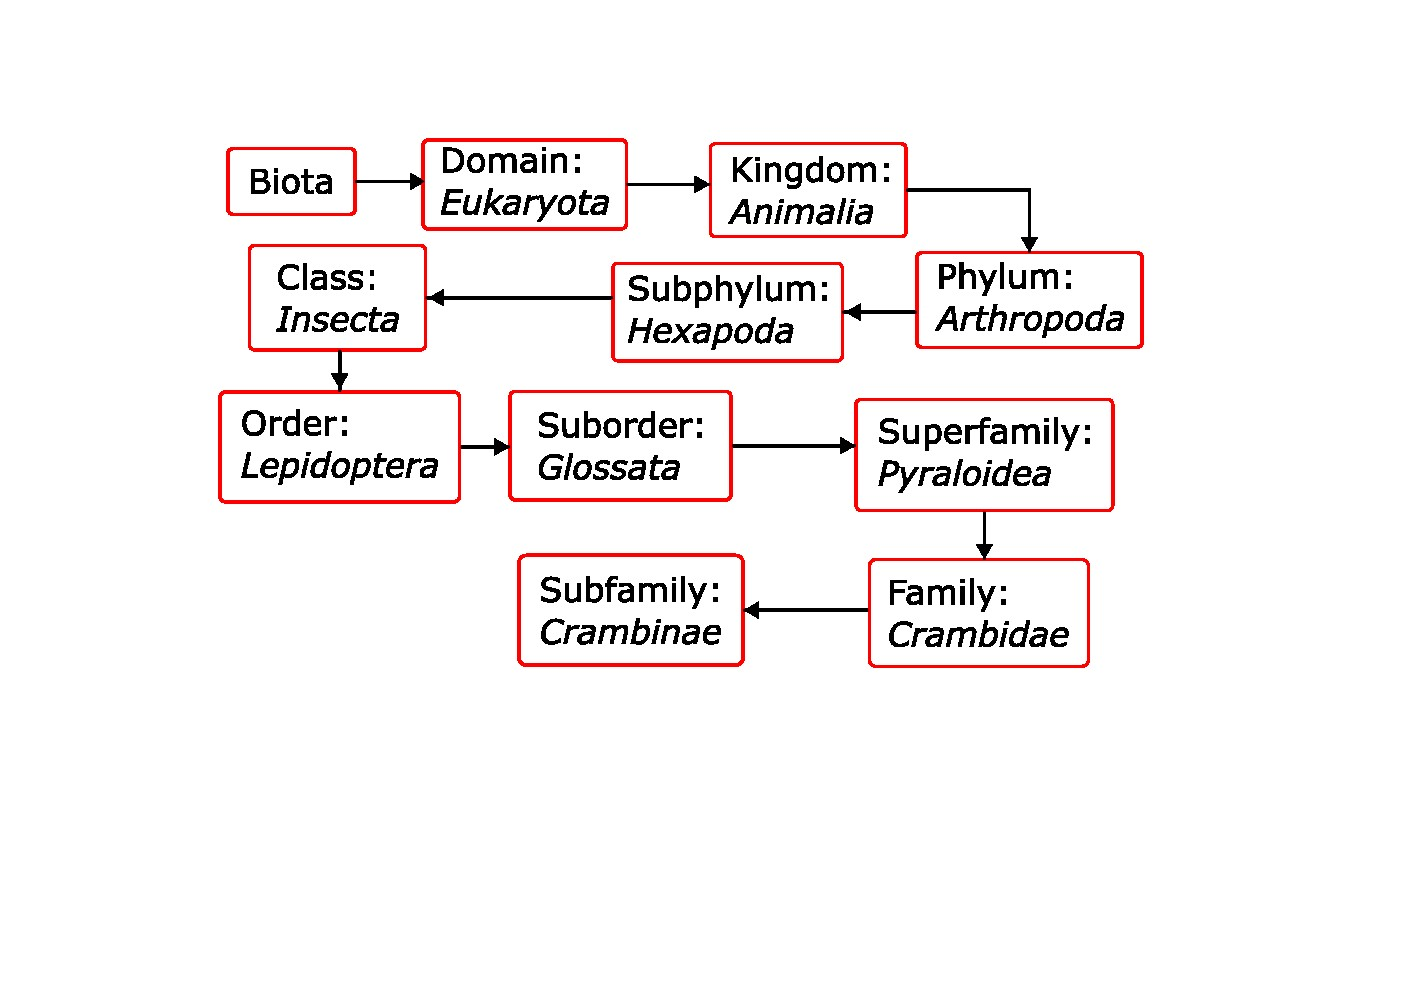
\includegraphics{./images/subfamily.jpg}
\caption{\emph{The Natural History Museum futher subdivide this group
into tribes, but these do not seem to be in general use}.}
\end{figure}
\end{column}
\end{columns}
\end{frame}

\begin{frame}{Confirming the ID}
\protect\hypertarget{confirming-the-id}{}
\begin{columns}[T]
\begin{column}{0.5\textwidth}
\begin{itemize}
\tightlist
\item
  We have gone as far as we can with external features.
\item
  The way forward is examination of the genitalia - \textbf{GenDet}.
\item
  We start by relaxing the dead moth
\end{itemize}
\end{column}

\begin{column}{0.5\textwidth}
\begin{figure}
\centering
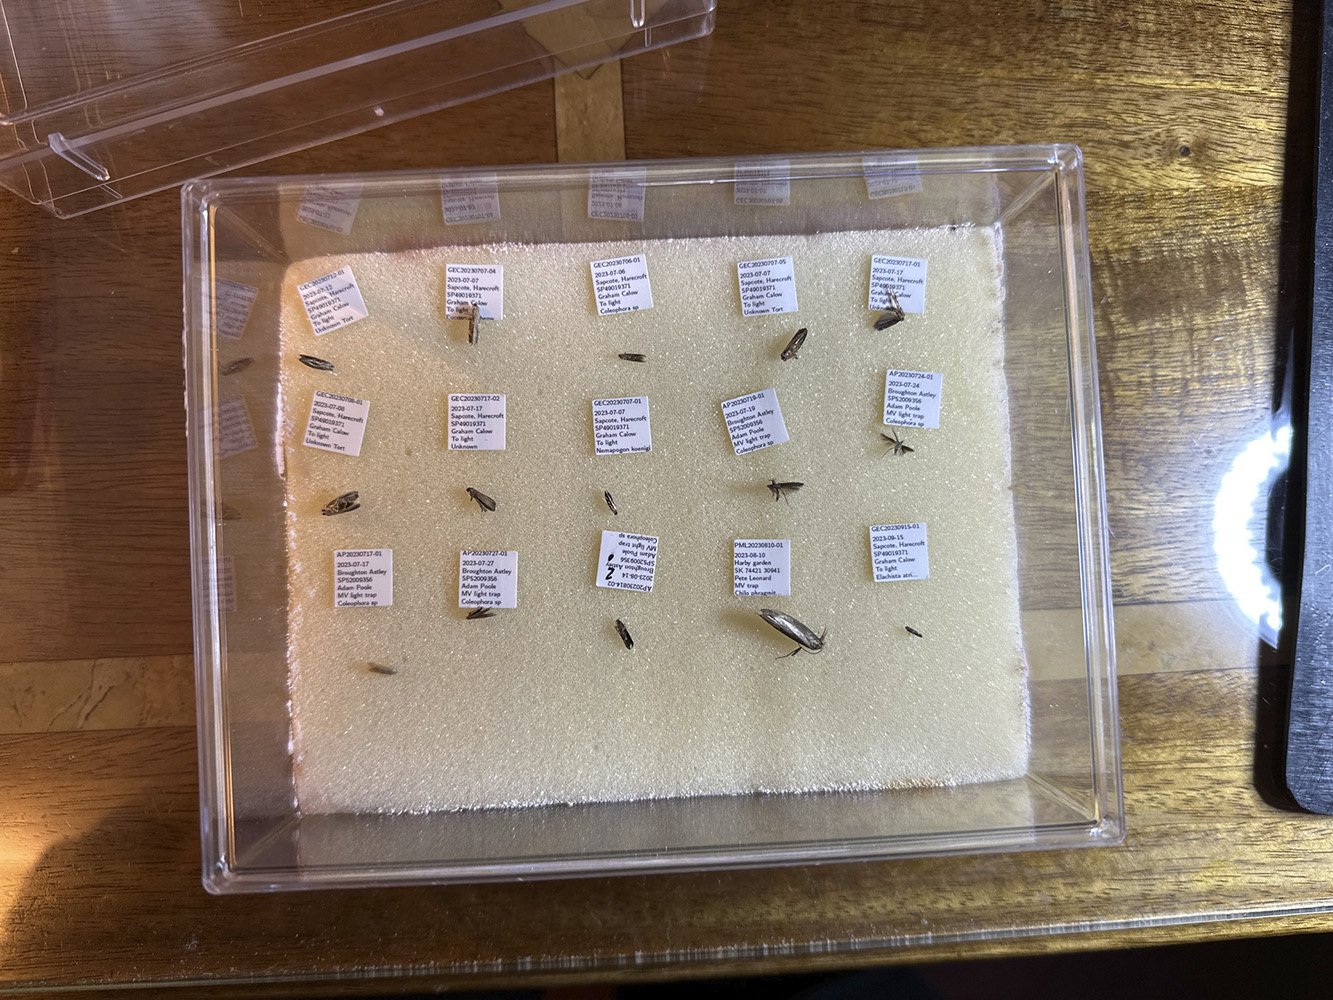
\includegraphics{./images/relaxing.jpg}
\caption{Relaxing chemicals are water based.}
\end{figure}
\end{column}
\end{columns}
\end{frame}

\begin{frame}{Setting}
\protect\hypertarget{setting}{}
\begin{columns}[T]
\begin{column}{0.5\textwidth}
\begin{itemize}
\tightlist
\item
  The relaxed moth is pinned and spread on a setting board.
\item
  Note how everything is carefully labelled.
\item
  It is then dried for a couple of weeks.
\item
  This process allows us to preserve as much of the specimen as
  possible.
\end{itemize}
\end{column}

\begin{column}{0.5\textwidth}
\begin{figure}
\centering
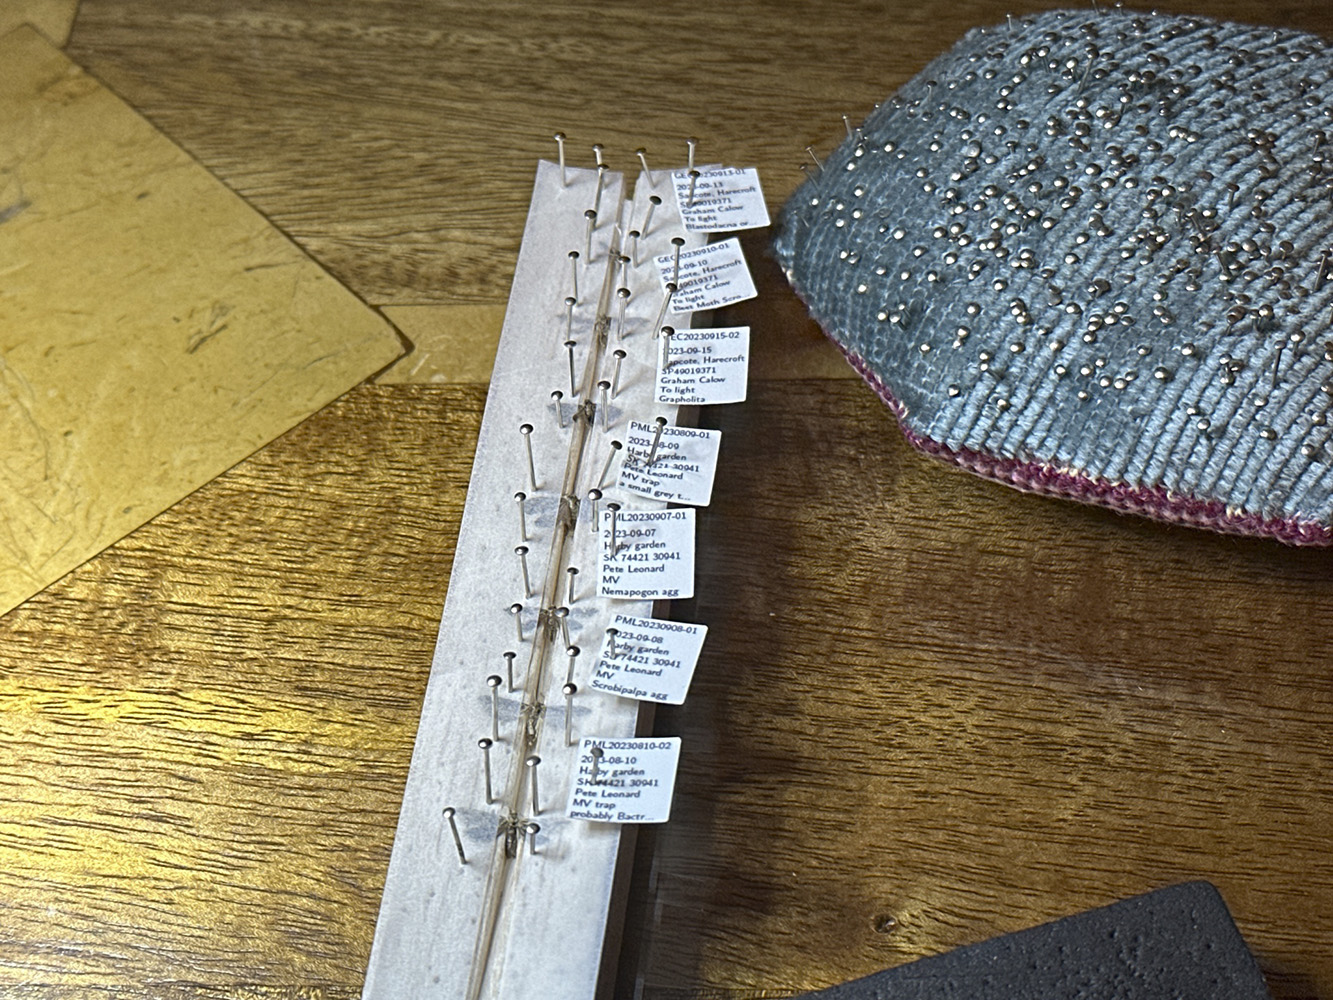
\includegraphics{./images/setting_moths.jpg}
\caption{A group of moths on the setting board.}
\end{figure}
\end{column}
\end{columns}
\end{frame}

\begin{frame}{We know it is a \textbf{Crambinae} (Grass Moth)}
\protect\hypertarget{we-know-it-is-a-crambinae-grass-moth}{}
\begin{columns}[T]
\begin{column}{0.5\textwidth}
\begin{itemize}
\tightlist
\item
  Date: 2021-07-25, VC55; Recorder: Pete Leonard; Size: FL 12 mm.
\item
  Could this be \emph{Pediasia contaminella} which is rare in VC55?
\item
  This specimen lacks the cross lines the dark point in the discal
  region typical of \emph{Pediasia contaminella}.
\item
  But \emph{Pediasia contaminella} said to have a distinctive upwards
  resting posture.
\end{itemize}
\end{column}

\begin{column}{0.5\textwidth}
\begin{figure}
\centering
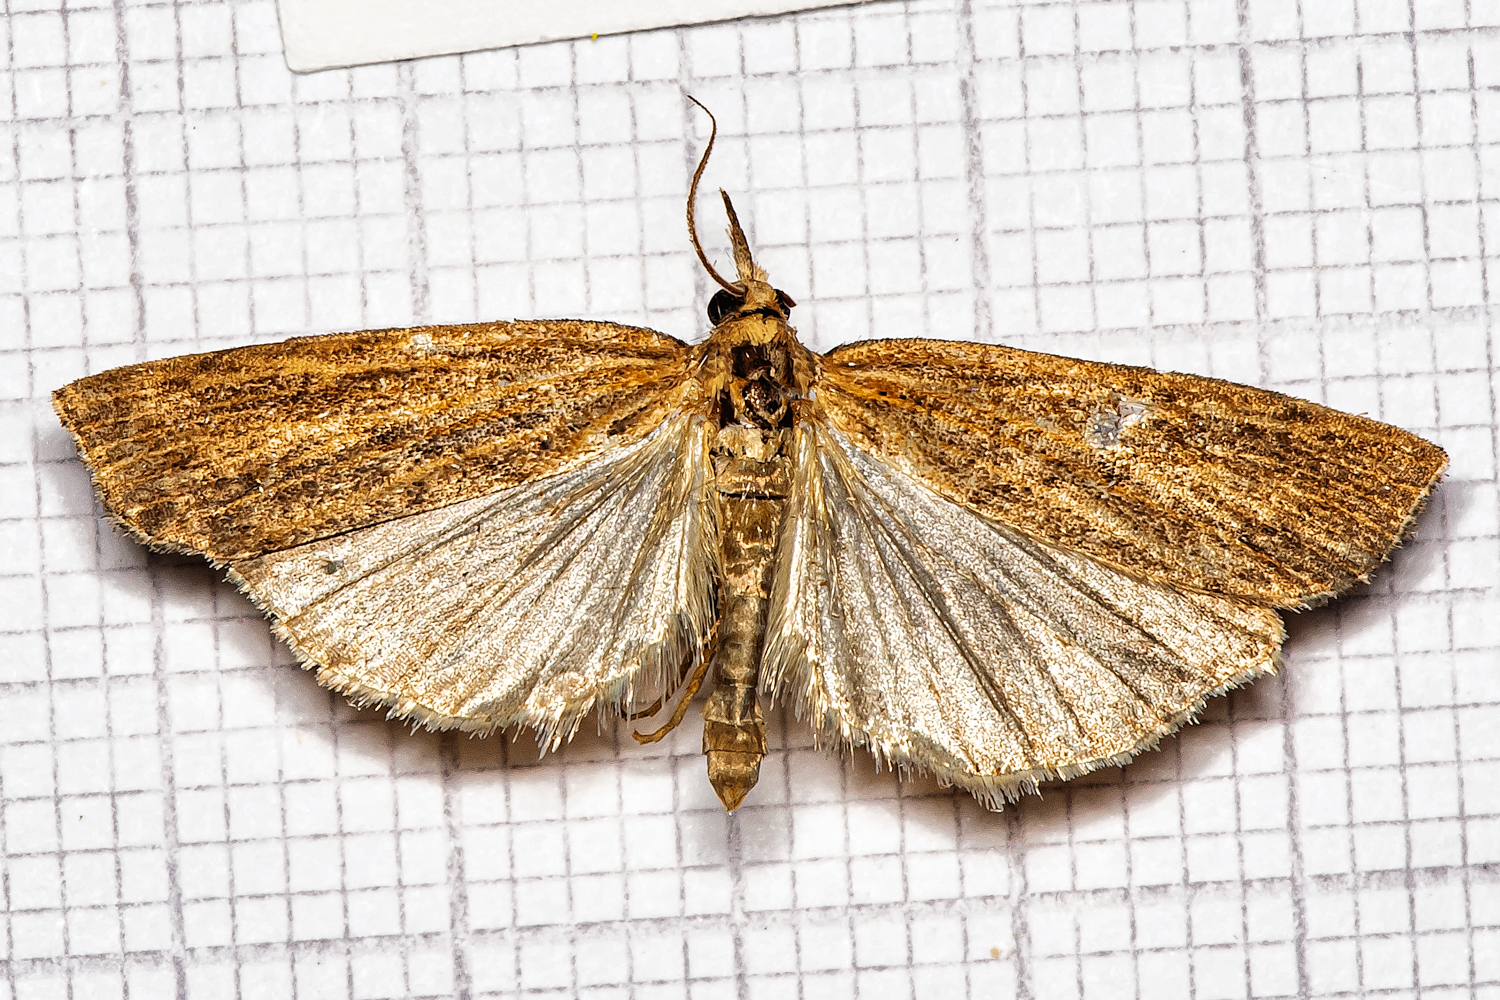
\includegraphics{./images/PJP20220218-0001a.jpg}
\caption{The set moth does not reveal any useful features for ID.}
\end{figure}
\end{column}
\end{columns}

Specimens seen in Sussex by PJP were all well marked and instantly
recognisable in both posture and appearance.
\end{frame}

\begin{frame}{Clarification}
\protect\hypertarget{clarification}{}
\begin{columns}[T]
\begin{column}{0.5\textwidth}
\begin{itemize}
\tightlist
\item
  The abdomen is removed from the moth and `cooked' for 30 minutes at 70
  degrees in 10\% KOH.
\item
  A label is place in the tube using paper and ink that can survive this
  process.
\item
  A body swap would be a disaster.
\end{itemize}
\end{column}

\begin{column}{0.5\textwidth}
\begin{figure}
\centering
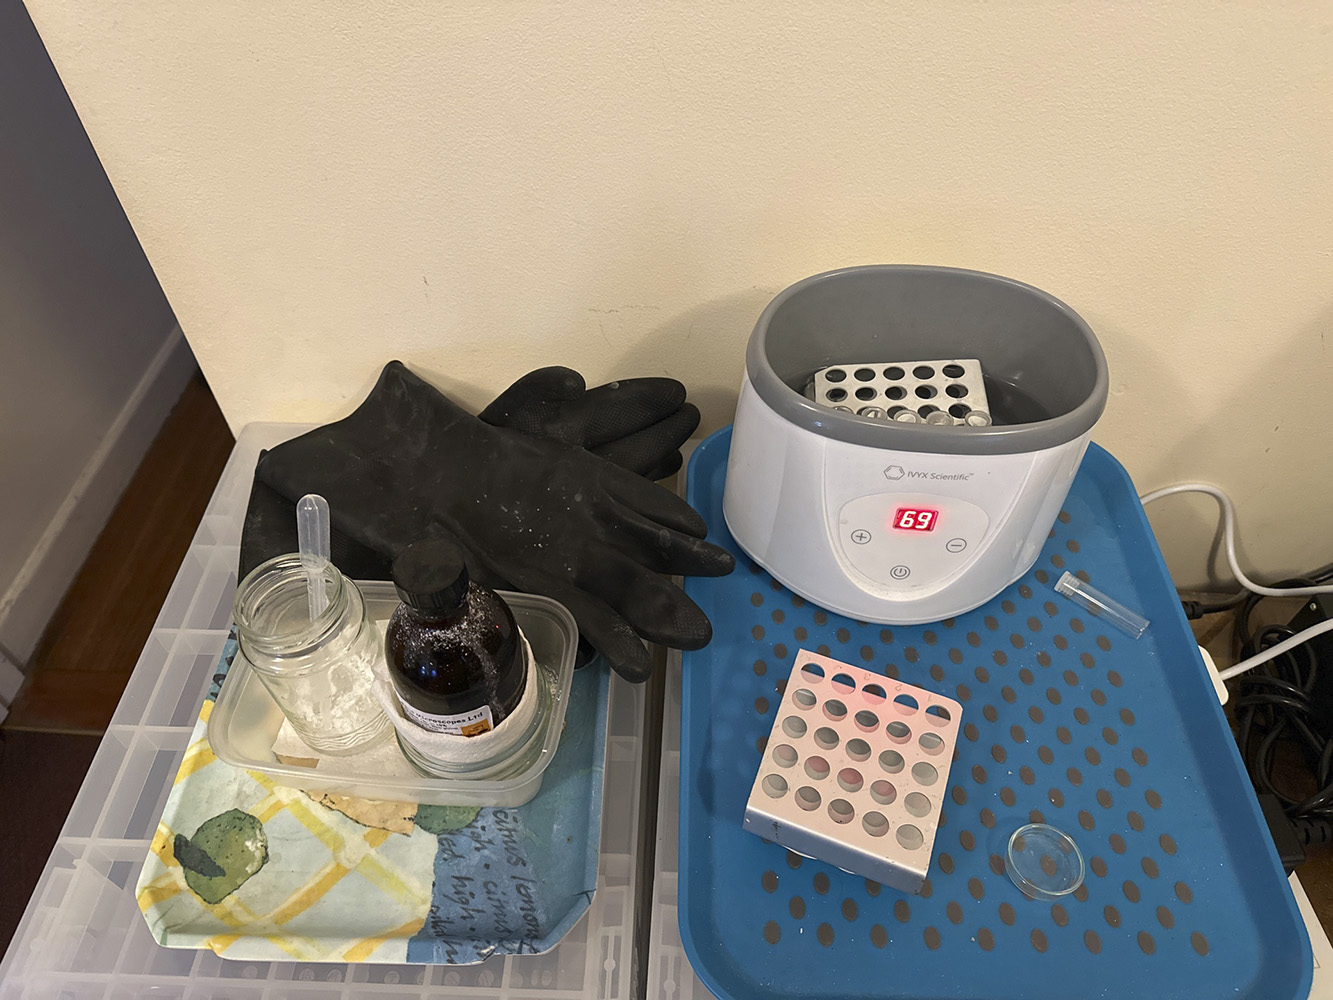
\includegraphics{./images/clarification.jpg}
\caption{Equiment used for clarification}
\end{figure}
\end{column}
\end{columns}

This process is loosely called \emph{clarification} as it dissolves the
soft tissues. Different authors use the term to describe rather
different processes.
\end{frame}

\begin{frame}{Dissecting}
\protect\hypertarget{dissecting}{}
\begin{columns}[T]
\begin{column}{0.5\textwidth}
\begin{itemize}
\tightlist
\item
  The genitalia are very small so a range of bought and homemade tools
  are used to dissect out the parts needed.
\item
  They are also very fragile, so you only get one chance on a moth this
  size.
\item
  No pressure when you are doing this for someone else!
\end{itemize}
\end{column}

\begin{column}{0.5\textwidth}
\begin{figure}
\centering
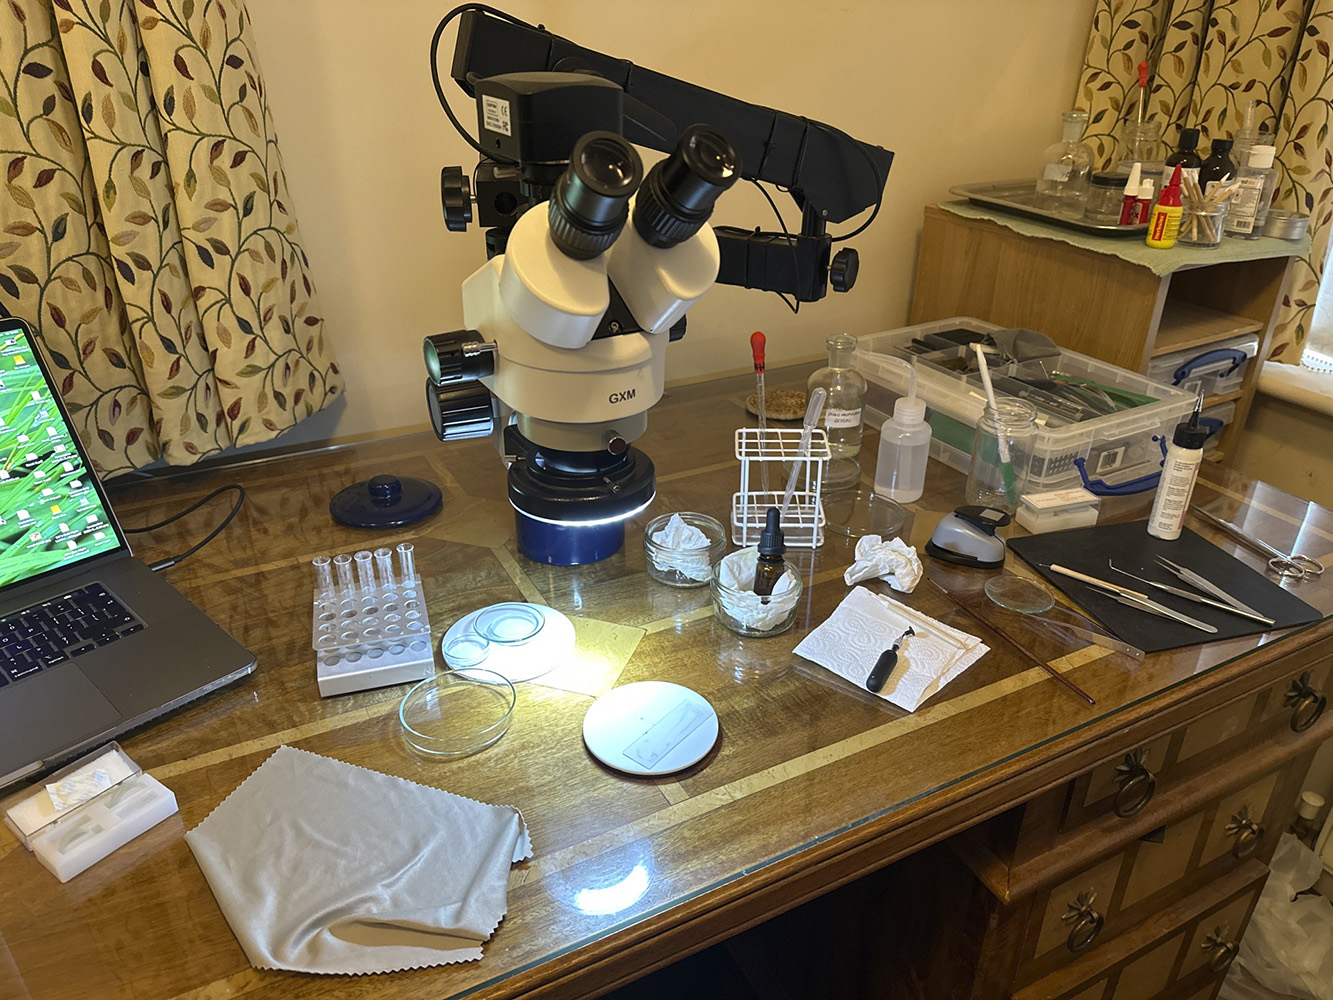
\includegraphics{./images/dissecting.jpg}
\caption{The smaller the dissection the more important the work space.}
\end{figure}
\end{column}
\end{columns}
\end{frame}

\begin{frame}{Mounting The Dissection}
\protect\hypertarget{mounting-the-dissection}{}
\begin{columns}[T]
\begin{column}{0.5\textwidth}
\begin{itemize}
\tightlist
\item
  The parts are washed in de-ionised water.
\item
  Soaked in a little aqueous mountant.
\item
  Placed on a slide and a coverslip placed on top.
\item
  Finally, a temporary label is glued to the slide
\end{itemize}
\end{column}

\begin{column}{0.5\textwidth}
\begin{figure}
\centering
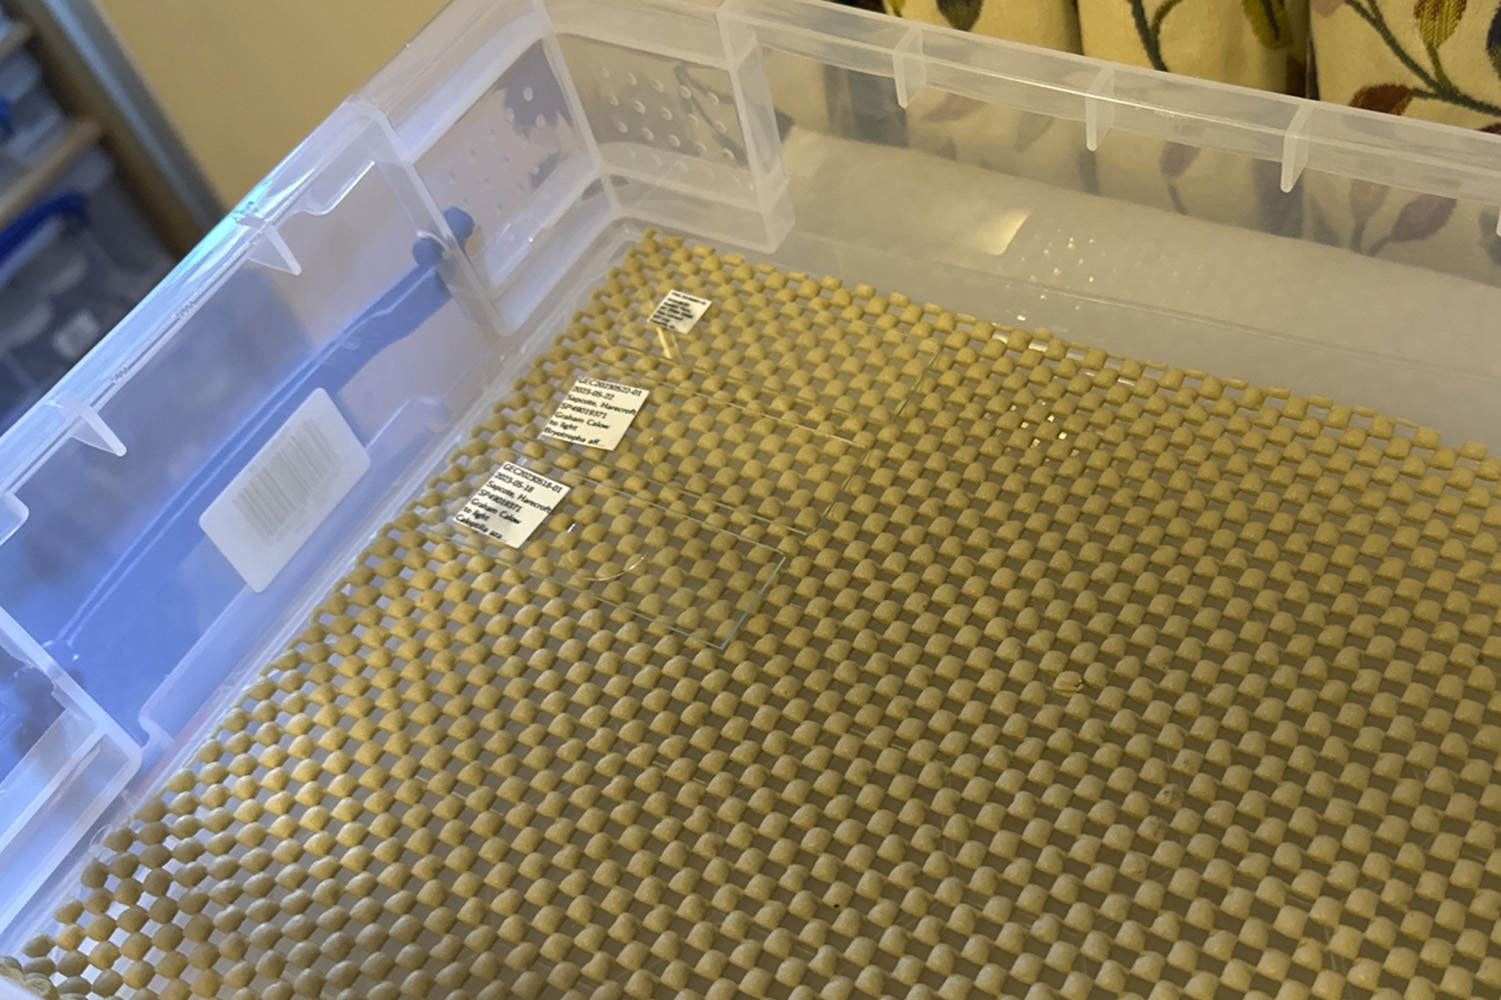
\includegraphics{./images/mounted_slides.jpg}
\caption{Slides are left for a few days to cure.}
\end{figure}
\end{column}
\end{columns}
\end{frame}

\begin{frame}{Ringing The Slide}
\protect\hypertarget{ringing-the-slide}{}
\begin{columns}[T]
\begin{column}{0.5\textwidth}
\begin{itemize}
\tightlist
\item
  Text
\item
  Text.
\item
  Text.
\end{itemize}
\end{column}

\begin{column}{0.5\textwidth}
\begin{figure}
\centering
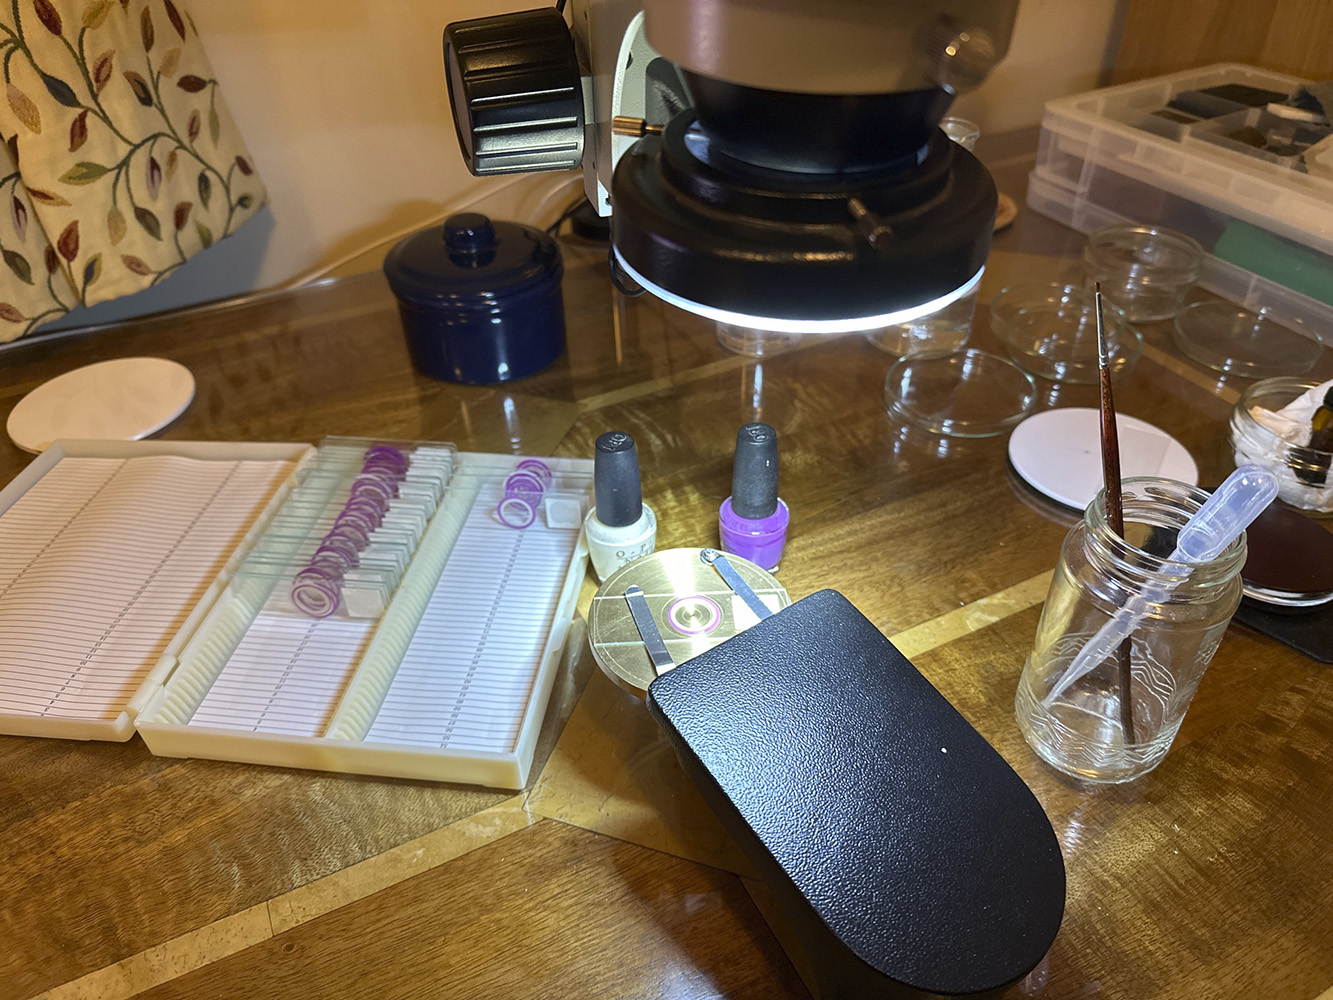
\includegraphics{./images/slideringing.jpg}
\caption{More text}
\end{figure}
\end{column}
\end{columns}
\end{frame}

\begin{frame}{Examination Under The Microscope}
\protect\hypertarget{examination-under-the-microscope}{}
\begin{columns}[T]
\begin{column}{0.5\textwidth}
\begin{itemize}
\tightlist
\item
  Text
\item
  Text.
\item
  Text.
\end{itemize}
\end{column}

\begin{column}{0.5\textwidth}
\begin{figure}
\centering
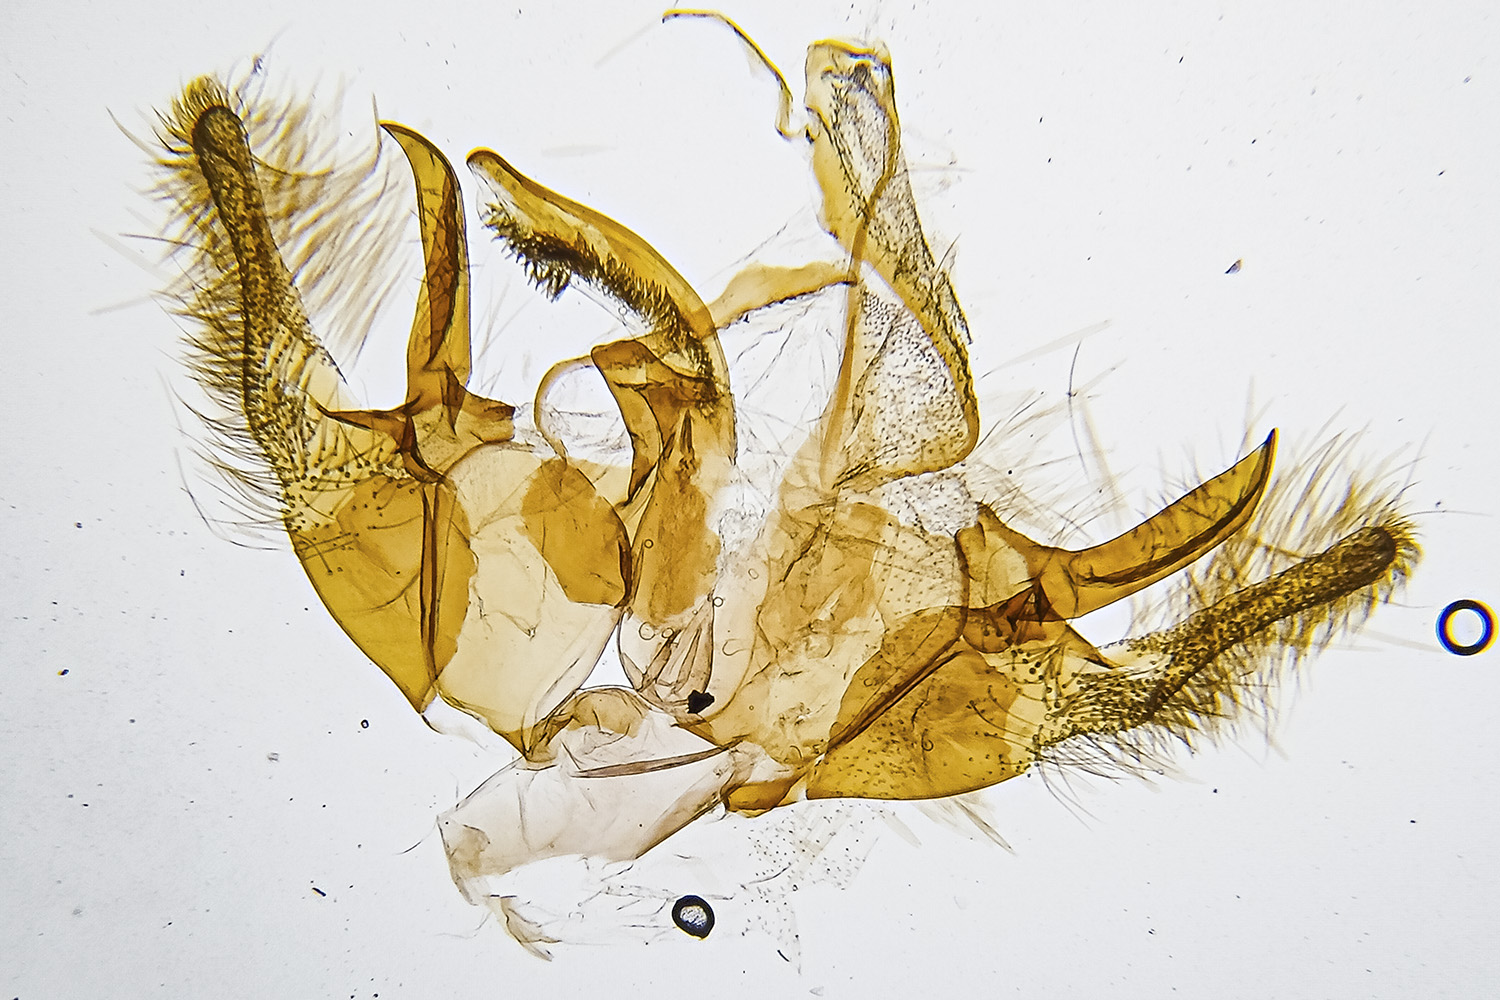
\includegraphics{./images/PJP20220218-001-raw-dissection.jpg}
\caption{Raw image}
\end{figure}
\end{column}
\end{columns}
\end{frame}

\begin{frame}{The Finished Dissection}
\protect\hypertarget{the-finished-dissection}{}
\begin{columns}[T]
\begin{column}{0.5\textwidth}
\begin{itemize}
\tightlist
\item
  Check the dissection against multiple sources as this specimen is not
  typical.
\item
  \url{https://mothdissection.co.uk}
\item
  \url{https://lepiforum.org}
\item
  Ask someone who is familiar with the species.
\end{itemize}
\end{column}

\begin{column}{0.5\textwidth}
\begin{figure}
\centering
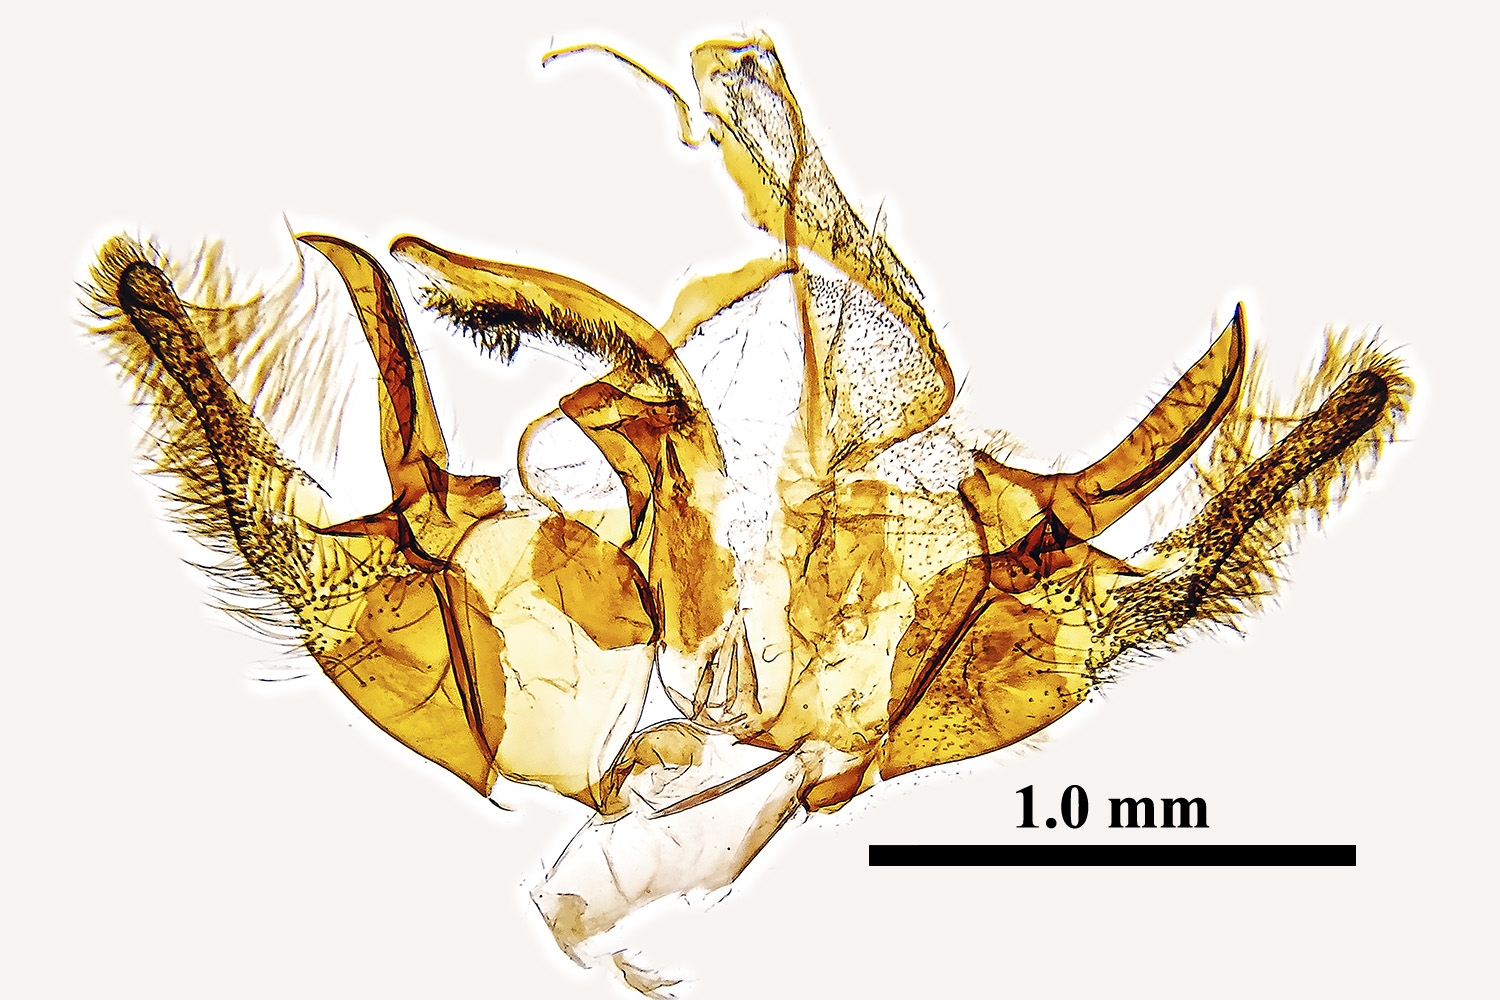
\includegraphics{./images/PJP20220218-001-developed-dissection.jpg}
\caption{Few keys for dissections.}
\end{figure}
\end{column}
\end{columns}
\end{frame}

\begin{frame}{Checking The ID}
\protect\hypertarget{checking-the-id}{}
\begin{columns}[T]
\begin{column}{0.5\textwidth}
\begin{itemize}
\tightlist
\item
  The dissection is compared with other close relatives.
\item
  We try to eliminate related species not on the UK list.
\item
  In this case we find no other candidates other than: \emph{Pediasia
  contaminella.}
\end{itemize}
\end{column}

\begin{column}{0.5\textwidth}
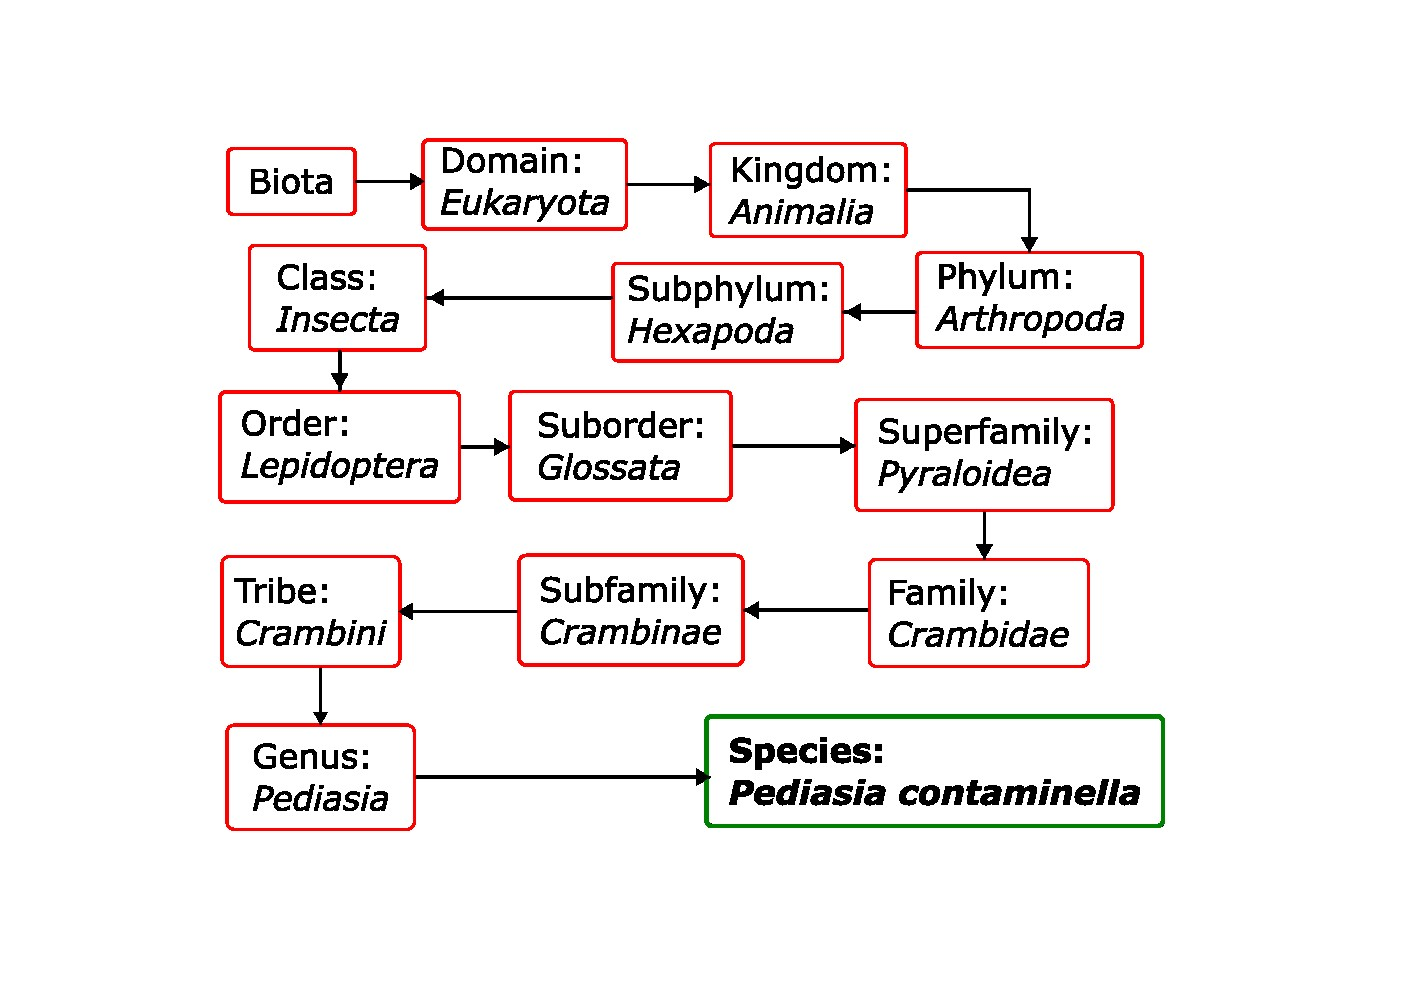
\includegraphics{./images/species.jpg}
\end{column}
\end{columns}
\end{frame}

\begin{frame}{To Recap}
\protect\hypertarget{to-recap}{}
\begin{columns}[T]
\begin{column}{0.5\textwidth}
\begin{itemize}
\tightlist
\item
  Identification of a tricky specimen is a tedious process.
\item
  Most of the time it turns out to be an unusual form of a common
  species as moths are very variable in size and wing pattern.
\item
  Environmental stress can cause size and colour variations.
\item
  Confirming the ID of something unusual requires the collation of a lot
  of evidence.
\end{itemize}
\end{column}

\begin{column}{0.5\textwidth}
\begin{figure}
\centering

\includegraphics{./images/placeholder.jpg}
\caption{More text}
\end{figure}
\end{column}
\end{columns}

\emph{But sometimes you get lucky!}
\end{frame}

\end{document}
